% !TeX spellcheck = en_GB
\documentclass{article}

\usepackage[utf8]{inputenc}
\usepackage{fancyhdr}
\usepackage{titlesec}
\usepackage{titling}
\usepackage{extramarks}
\usepackage{lastpage}
\usepackage{libertine}
\usepackage{ifthen}
\usepackage[
	a4paper,
	total={135mm, 240mm},
	includehead,
	headsep=12mm,
	footskip=15mm
]{geometry}
\usepackage{amsmath}
\usepackage{amsthm}
\usepackage{amssymb}
\usepackage{mathtools}
\usepackage{graphicx}
\usepackage{color}
\usepackage{cite}
\usepackage{listings}
\usepackage{xparse}
\usepackage{multirow}
\usepackage{xcolor}
\usepackage{booktabs}
\usepackage{bookmark}
\usepackage{draftfigure}
\usepackage{bbm}
\usepackage{tabularx}
\usepackage{verbatim}
\usepackage[ruled, vlined]{algorithm2e}

\definecolor{blue}{HTML}{1f77b4}
\definecolor{orange}{HTML}{ff7f0e}
\definecolor{green}{HTML}{2ca02c}
\definecolor{red}{HTML}{d62728}
\definecolor{purple}{HTML}{9467bd}
\definecolor{brown}{HTML}{8c564b}

% Custom commands

\DeclarePairedDelimiter\abs{\lvert}{\rvert}
\DeclareMathOperator{\E}{E}
\DeclareMathOperator{\Var}{Var}
\newcommand{\R}{\mathbb{R}}
\newcommand{\Z}{\mathbb{Z}}
\newcommand{\N}{\mathbb{N}}
\newcommand{\dd}{{\rm d}}
\newcommand{\eps}{\varepsilon}

\newcommand{\st} {\textsuperscript{st}}
\newcommand{\nd} {\textsuperscript{nd}}
\newcommand{\rd} {\textsuperscript{rd}}
\renewcommand{\th} {\textsuperscript{th}}

\NewDocumentCommand{\codeword}{v}{%
	\texttt{\textcolor{blue}{#1}}%
}

\newtheorem{theorem}{Theorem}[section]
\newtheorem{lemma}[theorem]{Lemma}

\newcommand{\metro}[7]{
	\begin{tabularx}{\linewidth}{@{}Xl@{}}
		\toprule[0.1em]
		Proposal distr. &#1\\
		Initialisation &#2\\
		Sample size &#3\\
		\midrule[0.1em]
		Traceplots	&\raisebox{%
				3mm - \totalheight}{%
				\includegraphics[width=0.8\linewidth]{#4}}\\
		Histograms &\raisebox{%
			3mm - \totalheight}{%
			\includegraphics[width=0.8\linewidth]{#5}}\\
		Accept. rates &#6\\
		%Means&#7\\ 
		\bottomrule[0.1em]
	\end{tabularx}
}

\newcommand{\metroall}[3]{
	\begin{table*}
		\centering
		\renewcommand{\arraystretch}{1.2}
		\input{../mcmc-tables/#1-QD-prior.txt}
		\caption{Metropolis algorithm for
			$\pi_{\theta}^{\text{QD}}$ for #3}
		\label{table:#1-1}
	\end{table*}
	
	\begin{table*}
		\centering
		\renewcommand{\arraystretch}{1.2}
		\input{../mcmc-tables/#1-QD-post.txt}
		\caption{Metropolis algorithm for
			$\pi^{\text{QD}}_{\theta \mid \mathbf{x}^{\text{#2}}}$ for #3}
	\end{table*}
	
	\begin{table*}
		\centering
		\renewcommand{\arraystretch}{1.2}
		\input{../mcmc-tables/#1-ME-prior.txt}
		\caption{Metropolis algorithm for
			$\pi_{\theta}^{\text{ME}}$ for #3}
	\end{table*}
	
	\begin{table*}
		\centering
		\renewcommand{\arraystretch}{1.2}
		\input{../mcmc-tables/#1-ME-post.txt}
		\caption{Metropolis algorithm for
			$\pi^{\text{ME}}_{\theta \mid \mathbf{x}^{\text{#2}}}$ for #3}
	\end{table*}
	
	\begin{table*}
		\centering
		\renewcommand{\arraystretch}{1.2}
		\input{../mcmc-tables/#1-ULS-post.txt}
		\caption{Metropolis algorithm for
			$\pi^{\text{ULS}}_{\theta \mid \mathbf{x}^{\text{#2}}}$ for #3}
		\label{table:#1-2}
	\end{table*}

	\begin{table*}
		\centering
		\renewcommand{\arraystretch}{1.2}
		\input{../mcmc-tables/#1-SAS-prior.txt}
		\caption{Metropolis algorithm for
			$\pi_{\theta}^{\text{SAS}}$ for #3}
		\label{table:#1-1}
	\end{table*}
	
	\begin{table*}
		\centering
		\renewcommand{\arraystretch}{1.2}
		\input{../mcmc-tables/#1-SAS-post.txt}
		\caption{Metropolis algorithm for
			$\pi^{\text{SAS}}_{\theta \mid \mathbf{x}^{\text{#2}}}$ for #3}
	\end{table*}
}

\newcommand{\marginals}[6]{
	\begin{table*}
		\centering
		\renewcommand{\arraystretch}{1.2}
		\begin{tabular}{@{}cc@{}}
			\toprule[0.1em]
			\raisebox{%
					-\totalheight}{%
					\includegraphics[%
						width=\linewidth]{%
						../plots/#1-#3-#6-0-marg.pdf}} \\
			\midrule[0.1em]
			\raisebox{%
					-\totalheight}{%
					\includegraphics[%
						width=\linewidth]{%
						../plots/#1-#3-#6-1-marg.pdf}} \\
			\midrule[0.1em]
			\raisebox{%
					-\totalheight}{%
					\includegraphics[%
						width=\linewidth]{%
						../plots/#1-#3-#6-2-marg.pdf}} \\
			\bottomrule[0.1em]
		\end{tabular}
		\caption{Prior and posterior #5 marginals of #4
			for #2}
		\label{table:#1-#3-#5-marg}
	\end{table*}
}

\newcommand{\allmarginals}[2]{
	\marginals{#1}{#2}{theta}{$(q_1, q_2, q_3)$}{univariate}{0}
	\marginals{#1}{#2}{theta}{$(q_1, q_2, q_3)$}{bivariate}{1}
	\marginals{#1}{#2}{q}{$(\mu, \log \sigma, \xi)$}{univariate}{0}
	\marginals{#1}{#2}{q}{$(\mu, \log \sigma, \xi)$}{bivariate}{1}
}

\newcommand{\allreturnlevels}[2]{
	\begin{table*}
		\centering
		\renewcommand{\arraystretch}{1.2}
		\begin{tabular}{@{}ccc@{}}
			\raisebox{-\totalheight}{%
				\includegraphics[%
					width=0.46\linewidth]{%
					../plots/#1-post-0-return-level.pdf}}
				&\raisebox{%
					-\totalheight}{%
					\includegraphics[%
						width=0.45\linewidth]{%
						../plots/#1-post-1-return-level.pdf}} \\
			\raisebox{-\totalheight}{%
				\includegraphics[%
					width=0.46\linewidth]{%
					../plots/#1-post-2-return-level.pdf}}
				&\raisebox{%
					-\totalheight}{%
					\includegraphics[%
						width=0.45\linewidth]{%
						../plots/#1-post-3-return-level.pdf}} \\
			\raisebox{-\totalheight}{%
				\includegraphics[%
					width=0.46\linewidth]{%
					../plots/#1-post-4-return-level.pdf}}
				&\raisebox{%
					-\totalheight}{%
					\includegraphics[%
						width=0.45\linewidth]{%
						../plots/#1-post-5-return-level.pdf}} \\
		\end{tabular}
		\caption{Mean return level with 95\% credibility intervals
			estimated using posterior distributions of
			$\pi^{\text{QD}}$ {\color{blue} \textbf{(blue)}},
			$\pi^{\text{ME}}$ {\color{orange} \textbf{(orange)}},
			$\pi^{\text{ULS}}$ {\color{green} \textbf{(green)}},
			and $\pi^{\text{SAS}}$ {\color{red} \textbf{(red)}},
			with analytic return level {\color{black} \textbf{(black solid)}},
			simulated return level {\color{black} \textbf{(black dashed)}}
			and empirical quantiles {\color{black} \textbf{(black dots)}}
			for #2}
		\label{table:#1-post-return-level}
	\end{table*}
}

%%% Style

\newcommand{\hwtitle}{Report version 8}
\newcommand{\hwdate}{21\th June 2020}
\newcommand{\hwname}{Tony Zheng}

\title{%
	\vspace{-15mm}\Huge{\hwtitle}\\
	\Large\vspace{1mm}\hwname\\
	\Large\vspace{1mm}\small{\itshape\hwdate}\vspace{-15mm}}
\date{}
\author{}

\pagestyle{fancy}
\lhead{\hwname}
\chead{\hwtitle}
\rhead{\firstxmark}
\lfoot{\lastxmark}
\cfoot{}
\rfoot{Page\ \thepage\ of\ \pageref{LastPage}}
\renewcommand\headrulewidth{0.4pt}
\renewcommand\footrulewidth{0.4pt}

\fancypagestyle{plain}{%
	\renewcommand{\headrulewidth}{0pt}%
	\fancyhf{}%
	\lfoot{\lastxmark}
	\cfoot{}
	\rfoot{Page\ \thepage\ of\ \pageref{LastPage}}
}

\allowdisplaybreaks

\begin{document}
%	
\maketitle
%
\section{Introduction}
%

%
The study of environmental conditions is crucial
in the development of large scale construction projects.
In particular, the study of long term behaviour
of environmental variables is necessary to understand
the risks of hazardous meteorological events such as
floods, storms and droughts.
This can be done using the well established theory of extreme values,
using asymptomatic models such as a Process point process model
described in Coles~\cite{coles2001}.
However, the analysis of extreme events is often hindered
by a scarcity of data, and an inadequate treatment
of model and prediction uncertainties.
To overcome these problems, a Bayesian methodology has been proposed.
This approach allows us to exploit prior information,
and provides a framework for taking account of the various uncertainties
in the prediction process.
%

%
A review of the use of Bayesian methods in extreme value theory
has been carried out in Coles and Powell~\cite{coles1996review},
and analyses of rainfall data have been performed
in both Coles et al.~\cite{coles2003} and Coles et al.~\cite{coles1996}.
In the latter, Coles et al. use the Poisson point process model,
and elicit expert-specified prior information
in the form of independent Gamma distributions
on the difference of three quantiles of the annual maxima.
In this paper, we will attempt to replicate this analysis using alternative prior distributions.
%

%
In \S~\ref{section:model}, we will outline the Poisson point process model.
In \S~\ref{section:priors}, we will describe the original prior distribution
used by Coles et al., and propose alternative prior distributions.
In \S~\ref{section:mcmc}, we will explain how Markov chain Monte Carlo (MCMC)
methods can be used in the analysis to avoid intractable calculations.
to sample from the
Finally, in \S~\ref{section:studies}, we will implement and compare our priors
in two simulation studies.
%
\section{Likelihood model}
\label{section:model}
%

%
Assume that we have daily observations
of some strictly positive random variable $X$ over $M$ years,
and some (sufficiently large) threshold $u$.
Denote by $\mathbf{x}=( x_1, \dots, x_{n_u})$
the exceedances of our data by the threshold.
Using the Poisson point process characterisation
of extremes detailed in Coles~\cite{coles2001},
the likelihood of the data is
%
\begin{align}
	L(\mu, \sigma, \xi \mid \mathbf{x})
		= \exp \left(-M \Lambda[u, \infty)\right)
		\prod_{i = 1}^{n_u} \lambda(x_i) \,,
	\label{eq:likelihood}
\end{align}
%
with intensity function
%
\begin{align}
	\lambda(x) \coloneqq
	\begin{cases}
		\frac{1}{\sigma}
			\left\{1 + \xi \left(\frac{x - \mu}{\sigma}\right)\right\}_+
			^ {-\frac{\xi + 1}{\xi}}
			&\quad \text{if $\xi \neq 0$} \,,\\
		\frac{1}{\sigma}\exp(-\frac{x - \mu}{\sigma})
			&\quad \text{if $\xi = 0$} \,,
	\end{cases}
	\label{eq:GP}
\end{align}
%
and
% 
\begin{align}
	\Lambda[u, \infty) &\coloneqq \int_u ^ \infty \lambda(x) \, \dd x \\
	&=
		\begin{cases}
			\left\{1 + \xi \left(\frac{u - \mu}{\sigma}\right)\right\}_+
			^ {-\frac{1}{\xi}}
			&\quad \text{if $\xi \neq 0$} \,,\\
			\exp(-\frac{u - \mu}{\sigma})
			&\quad \text{if $\xi = 0$} \,.
		\end{cases}
	\label{eq:Lambda}
\end{align}
%

%
The parameters $\theta \coloneqq (\mu, \sigma, \xi)$ are defined in the set
%
\begin{align}
	\Theta \coloneqq \{(\mu, \sigma, \xi) \in \R^3 \colon \sigma > 0 \} \,,
	\label{eq:Theta}
\end{align}
%
and are known as Generalised Extreme Value (GEV) parameters.
This is because the annual maxima of the data follow a GEV distribution
with parameters $\mu, \sigma, \xi$:
%
\begin{align}
	\Pr(\max\{X_1,\dots,X_{365}\leq x\}) =
		\begin{cases}
			\exp\left(-\left\{1 + \xi
			\left(\frac{x - \mu}{\sigma}\right)\right\}_+
			^ {-\frac{1}{\xi}}\right)
			&\quad \text{if $\xi \neq 0$} \,,\\
			\exp(-\exp(-\frac{x - \mu}{\sigma}))
			&\quad \text{if $\xi = 0$} \,.
		\end{cases}
	\label{eq:GEV-CDF}
\end{align}
%
Inverting (\ref{eq:GEV-CDF}), we get the quantile function
%
\begin{align*}
	q(p \mid \mu, \sigma, \xi) &=
	\begin{cases}
		\mu + \frac{\sigma}{\xi} (\exp(s \xi) - 1)
			&\quad \text{if $\xi \neq 0$}\,,\\
		\mu + \sigma s
			&\quad \text{if $\xi = 0$} \,,
	\end{cases}
\end{align*}
%
where
\begin{align*}
s \coloneqq -\log(-\log(1 - p))\,.
\end{align*}
%
Of interest to us are the quantiles corresponding to very small probabilities.
The \textit{return level} of a \textit{return period} $r$ in years
is defined as the quantile $q(1 - 1 / r\mid \mu, \sigma, \xi)$.
%
\section{Eliciting prior information}
\label{section:priors}
%
In Bayesian methodology, we elicit prior information about the model in the form
of a distribution $\pi_\theta$ on $(\mu, \sigma, \xi)$.
In our case, we assume that this information arises from the opinion of an expert.
Unfortunately, it is not feasible to specify joint distribution of $(\mu, \sigma, \xi)$.
Instead, we will consider a prior for three quantiles of the annual maxima.
%

%
Let $0 < p_1 < p_2 < p_3 < 1$ be three probabilities,
and consider the corresponding quantiles
%
\begin{align*}
	(q_1, q_2, q_3) \in {\cal Q}
		\coloneqq \{(q_1, q_2, q_3) \in \R^3 \colon q_1 < q_2 < q_3\} \,,
	\label{eq:Q}
\end{align*}
%
defined by
%
\begin{align}
	q_i \coloneqq q(1 - p_i \mid \mu, \sigma, \xi)\,, \quad i = 1, 2, 3 \,.
\end{align}
%
A prior for $(q_1, q_2, q_3)$ is equivalent to a prior for $(\mu, \sigma, \xi)$
through the inverse of the transformation
%
\begin{align*}
	g \colon \Theta &\to {\cal Q} \\
	(\mu, \sigma, \xi) &\mapsto (q_{1}, q_{2}, q_{3}) \,.
\end{align*}
%
Using the change of variables formula,
%
\begin{align}
	\pi_\theta(\mu, \sigma, \xi)
		&= \pi_q(g(\mu, \sigma, \xi)) \abs{\det{J(g)(\mu, \sigma, \xi)}}
		\mathbbm{1}_{\sigma > 0} \,,
	\label{eq:change-of-variables-1}
\end{align}
%
where $J(g)$ is the Jacobian of $g$.
We will now derive an expression for the determinant. Recall that
%
\begin{align*}
	s_i = -\log(-\log(1 - p_i)) \,, \quad i = 1, 2, 3 
\end{align*}
%
and
%
\begin{align}
	q_i = \mu + \sigma \frac{\exp(s_i \xi) - 1}{\xi} \,, \quad i = 1, 2, 3 \,,
\end{align}
%
where we are assuming that $\xi \neq 0$. Therefore
%
\begin{align*}
	\frac{\dd q_{i}}{\dd \mu}(\mu, \sigma, \xi)
		&= 1 \,,\\
	\frac{\dd q_{i}}{\dd \sigma}(\mu, \sigma, \xi)
		&= \frac{\exp(s_i \xi) - 1}{\xi} \,,\\
	\frac{\dd q_{i}}{\dd \xi}(\mu, \sigma, \xi)
		&= \frac{\sigma(s_i \xi \exp(s_i \xi) -\exp(s_i \xi) + 1)}{\xi ^ 2} \,,
\end{align*}
%
and therefore
%
\begin{align*}
	\det J(\mu, \sigma, \xi)
		&= \frac{\sigma}{\xi ^ {3}} \left\vert
		\begin{matrix}
			1 &1\\
			\exp(s_1 \xi)-1 &\exp(s_2 \xi)-1\\
			s_1 \xi \exp(s_1 \xi) - \exp(s_1 \xi) + 1
				&s_2 \xi \exp(s_2 \xi) - \exp(s_2 \xi) + 1
		\end{matrix}
	\right.\\
	&\qquad \qquad \left.
		\begin{matrix}
			1\\
			\exp(s_3 \xi) - 1\\
			s_3 \xi \exp(s_3 \xi) -\exp(s_3 \xi) + 1
		\end{matrix}
	\right\vert\\
	&= \frac{\sigma}{\xi ^ {3}} \abs*{
		\begin{matrix}
			1 &1 &1\\
			\exp(s_1 \xi) &\exp(s_2 \xi) &\exp(s_3 \xi)\\
			s_1 \xi \exp(s_1 \xi)
				&s_2 \xi \exp(s_2 \xi)
				&s_3 \xi \exp(s_3 \xi)
		\end{matrix}
	}\\
	&= \frac{\sigma}{\xi ^ {2}}
		\sum_{i=1}^3 s_i \exp(s_i \xi)
		(\exp(s_{i + 2} \xi) - \exp(s_{i + 1} \xi)) > 0 \,,
\end{align*}
%
where $i \equiv j \mod 3$ implies $s_i=s_j$.
Therefore the formula (\ref{eq:change-of-variables-1}) becomes
%
\begin{align}
	\pi_\theta(\mu, \sigma, \xi)
		&= \pi_q(g(\mu, \sigma, \xi)) \sigma \Psi(\xi)
		\mathbbm{1}_{\sigma>0} \,,
	\label{eq:change-of-variables-2}
\end{align}
%
with
%
\begin{align*}
	\Psi(\xi) \coloneqq \frac{1}{\xi^ {2}}
		\sum_{i=1}^3 s_i \exp(s_i \xi)
		(\exp(s_{i + 2} \xi) - \exp(s_{i + 1} \xi)) \,.
\end{align*}
%

%
As the data are assumed to be strictly positive,
the support of the quantiles implies
that a distribution for $(q_1, q_2, q_3)$ is a valid prior if and only if
%
\begin{align*}
	\Pr(0 < q_1 < q_2 < q_3) = 1\,.
\end{align*}
%
In order to satisfy this constraint,
Coles et al.~\cite{coles1996} specify marginal priors for the quantile differences
%
\begin{align*}
	\tilde{q}_1 &\coloneqq q_1 \,,\\
	\tilde{q}_2 &\coloneqq q_2 - q_1 \,,\\
	\tilde{q}_3 &\coloneqq q_3 - q_2 \,,
\end{align*}
%
and construct a joint distribution using an independent copula.
In particular, the expert provided $0.5$-quantile and $0.9$-quantile estimates
of each distribution, and Gamma distributions were fitted.
We will denote this prior $\pi^{\text{QD}}$ for Quantile Differences.
%

%
The choice of a distribution for the quantile differences can be motivated
using the principle of maximum entropy,
which was introduced by Jaynes~\cite{jaynes1957}.
Entropy is a measure of how much information we have about a distribution.
It is defined by Shannon~\cite{shannon1948}, for a continuous probability density $p$, as
%
\begin{align*}
	{\cal E}(p) = -\int_{{\cal D}(p)} p(x) \log_2(p(x)) \, \dd x \,.
\end{align*}
%
According to the principle of maximum entropy,
if we are to choose a prior from a class of distributions satisfying
certain constraints,
then we should chose a distribution which maximises the entropy in that class,
as it will be the least informative.
As quantile differences are positive,
we are looking for distributions with the support constraint $(0, +\infty)$,
and functional constraints defined by certain quantities which are fixed by an expert.
The maximum entropy distributions for various fixed quantities are shown below:
%
\begin{align*}
	\centering
	\renewcommand{\arraystretch}{1.2}
	\begin{tabular}{@{}ccc@{}}
		\toprule[0.1em]
		Fixed quantities &Maximum entropy distribution\\
		\midrule[0.1em]
		Any number of quantiles &Does not exist \\
		1\st\ moment &Exponential \\
		1\st, 2\nd\ moments &Truncated normal \\
		\bottomrule[0.1em]
	\end{tabular}
\end{align*}
%
Specifying $0.5$ and $0.9$-quantiles, as in $\pi^{\text{QD}}$,
does not have a maximum entropy solution.
However, specifying the mean leads to an exponential distribution,
and specifying the mean and variance leads to a truncated normal distribution.
We will denote these priors $\pi^{\text{QDE}}$ and $\pi^{\text{QDTN}}$ respectively.
In order to implement and compare these priors,
we will first specify $0.5$ and $0.9$-quantiles and fit Gamma distributions,
then obtain the mean and variance of these Gamma distributions
as specifications of the mean and variance.
%

%
Although we have thus far been considering an independent copula due to simplicity,
the choice of copula is also one which can be made using
the principle of maximum entropy.
We will consider a prior $\pi^{\text{ME}}$ which is the joint distribution with
maximum entropy for fixed marginals $q_1, q_2, q_3$
satisfying $\Pr(q_1 < q_2 < q_3) = 1$.
This order constraint allows us to specify priors on the quantiles instead
of the quantile differences, which may be more convenient for the expert.
However, in order to compare this prior to $\pi^{\text{QD}}$, we will 
choose these priors as approximations of the marginals of $\pi^{\text{QD}}_q$
using numerical minimisation of the Kullback–Leibler divergence.
%

%
In the case that we are only able to elicit information on two quantile differences,
we will consider a prior $\pi^{\text{ULS}}$ (Uniform on Log Sigma) which includes an improper uniform prior on $\log(\sigma)$.
As the maximum entropy distribution with a compact support $[a, b]$ is uniform,
this prior may be thought of as the maximum entropy distribution
when $a$ and $b$ tend to $-\infty$ and $+\infty$ respectively.
%

%
Finally, we will consider a variant of $\pi^{\text{QD}}$ where $\xi$ has a non-zero probability to be zero. This will be denoted $\pi^{\text{SAS}}$ (Spike And Slab) due to the shape of the marginal of $\xi$.
%
\subsection{QD:
	Gamma priors for independent quantile differences}
%

%
\label{section:prior-qd}
%
Coles et al.~\cite{coles1996} specify Gamma priors for the quantile differences
%
\begin{align*}
	\tilde{q}_1 &\coloneqq q_1 \sim \Gamma(\alpha_1, \beta_1) \,,\\
	\tilde{q}_2 &\coloneqq q_2 - q_1 \sim \Gamma(\alpha_2, \beta_2) \,,\\
	\tilde{q}_3 &\coloneqq q_3 - q_2 \sim \Gamma(\alpha_3, \beta_3) \,,
\end{align*}
%
with shape and rate parametrisation,
and multiply these together to form a joint distribution
$\pi_{\tilde{q}}^{\text{QD}}$ with independent marginals.
This is then converted into a prior for the quantiles
$\pi_q^{\text{QD}}$ using the transformation
%
\begin{align*}
	(\tilde{q}_1, \tilde{q}_2, \tilde{q}_3)
		&\mapsto (\tilde{q}_1, \tilde{q}_1 + \tilde{q}_2, \tilde{q}_1
		+ \tilde{q}_2 + \tilde{q}_3)\\
	&=(q_1,q_2,q_3)\,.
\end{align*}
%
Explicitly, the prior for $(q_1, q_2, q_3)$ is given by
%
\begin{align}
	\pi^{\text{QD}}_q(q_{1}, q_{2}, q_{3})
		&= C q_{1} ^ {\alpha_1 - 1} \exp(-\beta_1 q_{1}) \nonumber\\
	&\ \phantom{=} \times \prod^{3}_{i=2} (q_{i}-q_{i - 1}) ^ {\alpha_i - 1}
		\exp(-\beta_i(q_i - q_{i - 1}))
		\mathbbm{1}_{0 < q_1 \leq q_2 \leq q_3} \,,
	\label{eq:prior-1}
\end{align}
%
where
%
\begin{align*}
C \coloneqq \prod_{i=1}^3 \frac{\beta ^ {\alpha_i}_i}{\Gamma(\alpha_i)} \,.
\end{align*}
%
Substituting (\ref{eq:prior-1}) into (\ref{eq:change-of-variables-2}) gives us
\begin{align*}
	\pi^{\text{QD}}_\theta(\mu, \sigma, \xi) 
		&=C q_1^{\alpha_1 - 1} \exp\left(-\beta_1 q_1\right)
		\prod^{3}_{i=2} \left(\sigma \frac{\exp(s_{i} \xi)
		- \exp(s_{i - 1}\xi)}{\xi}\right) ^ {\alpha_i - 1} \nonumber\\
	&\ \phantom{=} \times \exp\left(-\beta_i \sigma \frac{\exp(s_{i} \xi)
		- \exp(s_{i - 1}\xi)}{\xi}\right) \sigma \Psi(\xi)
		\mathbbm{1}_{{q_1} > 0} \mathbbm{1}_{\sigma > 0} \nonumber\\
	&=C q_1 ^ {\alpha_1 - 1} \exp\left(-\beta_1 q_1\right)
		\sigma ^ {\alpha_2 + \alpha_3 - 1} \prod^{3}_{i=2}
		\left(\frac{\exp(s_{i} \xi) - \exp(s_{i - 1}\xi)}{\xi}\right)
		^ {\alpha_i-1} \nonumber\\
	&\ \phantom{=} \times \exp\left(-\frac{\sigma}{\xi}
		\sum_{i=2}^3 \beta_i (\exp(s_{i} \xi) - \exp(s_{i-1} \xi))\right)
		\Psi(\xi) \mathbbm{1}_{{q_1} > 0}\mathbbm{1}_{\sigma > 0} \nonumber\\
	&=C q_1 ^ {\alpha_1 - 1} \exp\left(-\beta_1 q_1\right)
		\sigma ^ {\alpha_2 + \alpha_3 - 1} \Phi_1(\xi)
		\exp\left(-\sigma \Phi_2(\xi)\right) \mathbbm{1}_{{q_1} > 0}
		\mathbbm{1}_{\sigma > 0} \,,
\end{align*}
%
where
%
\begin{align*}
	\Psi(\xi) &= \frac{1}{\xi ^ {2}} \sum_{i=1}^3 s_i \exp(s_i \xi)
		(\exp(s_{i + 2} \xi) - \exp(s_{i + 1} \xi)) \,,\\
	\Phi_1(\xi) &\coloneqq \prod^{3}_{i=2} \left(\frac{\exp(s_{i} \xi)
		- \exp(s_{i - 1} \xi)}{\xi}\right) ^ {\alpha_i - 1} \Psi(\xi) \,,\\
	\Phi_2(\xi) &\coloneqq \frac{1}{\xi}
		\sum_{i=2}^3 \beta_i(\exp(s_{i} \xi) - \exp(s_{i - 1} \xi)) > 0 \,.
\end{align*}
%

%
The marginal of $(\sigma, \xi)$ is
%
\begin{align}
	\pi ^ {\text{QD}}_{\sigma, \xi}(\sigma, \xi)
		&= \int_{-\infty}^\infty \pi_{\theta}^{\text{QD}}(\mu, \sigma, \xi)
		\, \dd \mu \nonumber\\
	&=C \int_{0}^\infty q_1 ^ {\alpha_1 - 1} \exp\left(-\beta_1 q_1\right)
		\sigma^{\alpha_2 + \alpha_3 - 1} \Phi_1(\xi)
		\exp\left(-\sigma \Phi_2(\xi)\right)\mathbbm{1}_{\sigma > 0}
		\, \dd q_1 \nonumber\\
	&= C \sigma ^ {\alpha_2 + \alpha_3 - 1} \Phi_1(\xi)
		\exp\left(-\sigma \Phi_2(\xi)\right) \beta_1 ^ {-\alpha_1} \nonumber\\
	&\ \phantom{=} \times \int_{0}^\infty (\beta_1 q_1) ^ {\alpha_1 - 1}
		\exp\left(-\beta_1 q_1\right) \beta_1 \, \dd q_1
		\mathbbm{1}_{\sigma > 0} \nonumber\\
	&= C \sigma ^ {\alpha_2 + \alpha_3 - 1} \Phi_1(\xi)
		\exp\left(-\sigma \Phi_2(\xi)\right) \beta_1 ^ {-\alpha_1}
		\Gamma(\alpha_1) \mathbbm{1}_{\sigma > 0} \nonumber\\
	&= C_2 \sigma ^ {\alpha_2 + \alpha_3 - 1} \Phi_1(\xi)
		\exp\left(-\sigma \Phi_2(\xi)\right) \mathbbm{1}_{\sigma > 0} \,,
	\label{eq:prior-1-xi-sigma}
\end{align}
%
where
%
\begin{align*}
	C_2 = \frac{\beta_2 ^ {\alpha_2} \beta_3 ^ {\alpha_3}}
		{\Gamma(\alpha_2) \Gamma(\alpha_3)} \,.
\end{align*}
%
The marginal of $\xi$ is
%
\begin{align}
	\pi ^ {\text{QD}}_\xi(\xi)
		&= \int_{-\infty}^\infty \pi^{\text{QD}}_{\sigma, \xi}(\sigma, \xi)
		\, \dd \sigma \nonumber\\
	&=C_2 \int_{0}^\infty \sigma ^ {\alpha_2 + \alpha_3 - 1} \Phi_1(\xi)
		\exp\left(-\sigma \Phi_2(\xi)\right) \, \dd \sigma \nonumber\\
	&=C_2 \Phi_1(\xi) \Phi_2(\xi) ^ {-\alpha_2 - \alpha_3} \nonumber\\
	&\ \phantom{=} \times \int_{0}^\infty (\sigma \Phi_2(\xi))
		^ {\alpha_2 + \alpha_3 - 1} \exp\left(-\sigma \Phi_2(\xi)\right)
		\Phi_2(\xi) \, \dd \sigma \nonumber\\
	&= C_2 \Phi_1(\xi) \Phi_2(\xi) ^ {-\alpha_2 - \alpha_3}
		\Gamma(\alpha_2 + \alpha_3) \nonumber\\
	&=C_3 \frac{\Phi_1(\xi)}{\Phi_2(\xi) ^ {\alpha_2 + \alpha_3}} \,.
	\label{eq:prior-1-xi}
\end{align}
%
where
%
\begin{align*}
	C_3 = \frac{\Gamma(\alpha_2 + \alpha_3) \beta_2 ^ {\alpha_2}
		\beta_3 ^ {\alpha_3}} {\Gamma(\alpha_2) \Gamma(\alpha_3)} \,.
\end{align*}
%
\subsection{ME:
	Prior from maximum entropy distribution of quantiles}
\label{section:prior-me}
%

%
For this prior, we specify marginal priors on the quantiles
$q_1, q_2, q_3$ directly.
In particular, we choose Gamma distributions
%
\begin{align*}
	q_i \sim \Gamma(\alpha_i, \beta_i) \,, \quad i = 1, 2, 3
\end{align*}
%
with shape and rate parametrisation.
Let $f_i$ and $F_i$ be their PDFs and CDFs respectively. Let
%
\begin{align*}
	h_i(x) &= \frac{f_i(x)}{F_{i - 1}(x) - F_i(x)}\\
	&= \frac{\Gamma(\alpha_{i - 1})\beta_i ^ {\alpha_i} x ^ {\alpha_i - 1}
		\exp(-\beta_i x)}{\gamma(\alpha_{i - 1}, \beta_{i - 1} x)
		\Gamma(\alpha_{i}) - \gamma(\alpha_i, \beta_i x)\Gamma(\alpha_{i - 1})}
\end{align*}
%
if $x > 0$, and $h(x) = 0$ otherwise.
According to Butucea et al.~\cite{butucea2018},
under certain conditions on the $F_i$,
the joint distribution of $(q_1, q_2, q_3)$ with maximum entropy
which satisfies $\Pr(q_1 \leq q_2 \leq q_3) = 1$ has the unique density
%
\begin{align*}
	\pi^{\text{ME}}_q(q_1, q_2, q_3) &= f_1(q_1) \prod_{i=2}^3 h_i(q_i)
		\exp\left(-\int_{q_{i - 1}}^{q_i} h_i(s) \, \dd s\right)
		\mathbbm{1}_{q_1 \leq q_2 \leq q_3}\\
	&=\frac{\beta_1 ^ {\alpha_1}}{\Gamma(\alpha_1)} {q_1} ^ {\alpha_1 - 1}
		\exp(-\beta_1 q_1)\prod_{i=2}^3 h_i(q_i)
		\exp\left(-\int_{q_{i - 1}}^{q_i} h_i(s) \, \dd s\right)
		\mathbbm{1}_{0 < q_1 \leq q_2 \leq q_3} \,.
\end{align*}
%
See \S~\ref{section:C2} for more detail on one of these conditions.
This distribution can be obtained in Python using the class
\codeword{MaximumEntropyOrderStatisticsDistribution}
from the library OpenTURNS~\cite{OpenTURNS}.
Therefore, from equation (\ref{eq:change-of-variables-2}),
the corresponding prior on the GEV parameters becomes
%
\begin{align}
	\pi^{\text{ME}}_\theta(\mu, \sigma, \xi)
		&=\frac{\beta_1 ^ {\alpha_1}}{\Gamma(\alpha_1)} {q_1}^{\alpha_1 - 1}
		\exp(-\beta_1 q_1) \prod_{i=2}^3 h_i(q_i)
		\exp\left(-\int_{q_{i - 1}}^{q_i} h_i(s) \, \dd s\right)
		\sigma \Psi(\xi) \mathbbm{1}_{q_1 > 0} \mathbbm{1}_{\sigma > 0} \,,
\end{align}
%
where
%
\begin{align*}
	\Psi(\xi) = \frac{1}{\xi ^ {2}} \sum_{i = 1}^3 s_i \exp(s_i \xi)
		(\exp(s_{i + 2}\xi) - \exp(s_{i + 1} \xi)) \,.
\end{align*}
%
\subsection{ULS: Uniform prior on log sigma}
%

%
This is a variant of $\pi^{\text{QD}}$,
in which an improper uniform prior is specified for $\log \sigma$,
and Gamma priors are specified for independent quantile differences
$\tilde{q}_1$ and $\tilde{q}_2$ given $\sigma$. That is,
%
\begin{align*}
	\pi^{\text{ULS}}_{\sigma}(\sigma)
		&\propto \frac{1}{\sigma} \mathbbm{1}_{\sigma > 0} \,,\\
	\pi^{\text{ULS}}_{q_1, q_2 \mid \sigma}(q_{1}, q_{2} \mid \sigma)
		&\propto q_{1} ^ {\alpha_1 - 1} \exp(-\beta_1 q_{1})
		(q_{2} - q_{1}) ^ {\alpha_2 - 1} \exp(-\beta_2 (q_2 - q_{1}))
		\mathbbm{1}_{0 <q_1 \leq q_2}\\
	\implies \pi^{\text{ULS}}_{\sigma, q_1, q_2}(\sigma, q_1, q_2)
		&\propto q_{1} ^ {\alpha_1 - 1} \exp(-\beta_1 q_{1})
		(q_{2} - q_{1}) ^ {\alpha_2 - 1} \exp(-\beta_2(q_2 - q_{1}))
		\frac{1}{\sigma} \mathbbm{1}_{\sigma > 0}
		\mathbbm{1}_{0 < q_1 \leq q_2} \,.
\end{align*}
%
Using the inverse transformation
%
\begin{align*}
	g \colon (\mu, \sigma, \xi) &\mapsto (\sigma, q_{1}, q_{2})
\end{align*}
%
whose determinant of the Jacobian is
%
\begin{align*}
	\det J(g) = \frac{\sigma}{\xi ^ {2} }
		((s_1 \xi - 1) \exp(s_1 \xi) - (s_2 \xi - 1) \exp(s_2 \xi)) \,,
\end{align*}
%
the prior on $(\mu, \sigma, \xi)$ can be expressed as
%
\begin{align*}
	\pi^{\text{ULS}}_\theta(\mu, \sigma, \xi)
		&\propto q_{1} ^ {\alpha_1 - 1} \exp(-\beta_1 q_{1})
		\sigma ^ {\alpha_2 - 1} \left(\frac{\exp(s_{2} \xi)
		- \exp(s_{1} \xi)} {\xi}\right) ^ {\alpha_2 - 1}\\
	&\ \phantom{=} \times \exp\left(-\beta_2 \sigma \frac{\exp(s_{2} \xi)
		- \exp(s_{1} \xi)}{\xi}\right) \Psi(\xi)
		\mathbbm{1}_{\sigma, q_1 > 0} \,,
\end{align*}
%
with
%
\begin{align*}
	\Psi(\xi) \coloneqq \frac{1}{\xi ^ {2}} \abs{(s_1 \xi - 1) \exp(s_1 \xi)
		- (s_2 \xi - 1) \exp(s_2 \xi))} \,.
\end{align*}
%
The posterior, with a single observation $x$ such that
%
\begin{align*}
1 + \xi \left(\frac{x - \mu}{\sigma}\right) > 0 \,,
\end{align*}
%
is written
%
\begin{align*}
	\pi^{\text{ULS}}_{\theta\mid x}(\mu, \sigma, \xi \mid x)
&\propto q_{1} ^ {\alpha_1 - 1} \exp(-\beta_1 q_{1})
	\sigma ^ {\alpha_2 - 1} \left(\frac{\exp(s_{2} \xi)
	- \exp(s_{1} \xi)} {\xi}\right) ^ {\alpha_2 - 1}\\
&\ \phantom{=} \times \exp\left(-\beta_2 \sigma \frac{\exp(s_{2} \xi)
	- \exp(s_{1} \xi)}{\xi}\right) \Psi(\xi)\\
&\ \phantom{=} \times \exp \left(-M \left\{1 + \xi
	\left(\frac{u - \mu}{\sigma}\right)\right\} ^ {-\frac{1}{\xi}}\right)
	\frac{1}{\sigma}
	\left\{1 + \xi \left(\frac{x - \mu}{\sigma}\right)\right\}
	^ {-\frac{\xi + 1}{\xi}}
	\mathbbm{1}_{\sigma, q_1 > 0} \,.
\end{align*}
%
In order to show that this is proper,
we need to show that the following is integrable:
%
\begin{align*}
	\pi^{\text{ULS}}_{\sigma\mid x, \mu, \xi}(\sigma \mid x, \mu, \xi) &\propto
		q_{1} ^ {\alpha_1 - 1} \exp(-\beta_1 q_{1}) \sigma ^ {\alpha_2 - 2}
		\exp\left(-\beta_2 \sigma \frac{\exp(s_{2} \xi)
			- \exp(s_{1} \xi)}{\xi}\right) \\
	&\ \phantom{=} \times \exp \left(-M \left\{1 + \xi
		\left(\frac{u - \mu}{\sigma}\right)\right\} ^ {-\frac{1}{\xi}}\right)
		\left\{1 + \xi \left(\frac{x - \mu}{\sigma}\right)\right\}
		^ {-\frac{\xi + 1}{\xi}}
		\mathbbm{1}_{\sigma, q_1 > 0} \,.
\end{align*}
%
Northrop and Attalides~\cite{northrop2016} show that for a GEV likelihood model
with at least 2 observations,
if uniform priors are specified for $\mu$ and $\log \sigma$,
and a proper prior is placed on $\xi$,
then the joint prior will yield a proper posterior.
%
\subsection{SAS: Spike-and-slab prior}
%

%
This is a prior with a non-zero probability mass (spike) at $\xi = 0$,
and a flat slab elsewhere.
%

%
We use the method proposed by Kuo and Mallick \cite{kuo1998}.
We introduce an indicator random variable $\gamma$ such that
$\gamma = 0$ when $\xi$ is ``in'' the spike
and $\gamma = 1$ when $\xi$ is ``in'' the slab.
The probability that $\xi$ is nonzero can then be calculated
as the mean of $\gamma$.
We also need a random variable $\beta$ such that $\xi = \beta \gamma$,
which determines the distribution of $\xi$ in the slab.
Our model now has parameters $\eta \coloneqq (\mu, \sigma, \beta, \gamma)$,
and we suppose that $\gamma$ does not depend on the other parameters.
%

%
If we have a prior $\pi_\theta$ for $(\mu, \sigma, \xi)$, then we can set
%
\begin{align*}
	\pi_{\mu, \sigma, \beta}^{\text{SAS}} &\coloneqq \pi_\theta \\
	\pi_\gamma^{\text{SAS}}(\gamma)
		&\coloneqq \alpha ^ \gamma (1 - \alpha) ^ {1 - \gamma} \\
	\implies \pi_{\eta}^{\text{SAS}}(\eta)
		&= \pi_\theta(\mu, \sigma, \beta)
		\alpha ^ \gamma (1 - \alpha) ^ {1 - \gamma} \,,
\end{align*}
%
with $\alpha \in [0, 1]$. The posterior is then proportional to
%
\begin{align*}
	\pi_{\eta \mid \mathbf{x}}^{\text{SAS}}(\eta \mid \mathbf{x}) &\propto
		L(\mu, \sigma, \beta \gamma \mid \mathbf{x})
		\pi_\theta(\mu, \sigma, \beta)
		\alpha ^ \gamma (1 - \alpha) ^ {1 - \gamma} \,.
\end{align*}
%

%
Since, up to the same constant of proportionality, we have
%
\begin{align*}
	\pi_{\gamma \mid \mu, \sigma, \beta, \mathbf{x}}^{\text{SAS}}
		(0 \mid \mu, \sigma, \beta, \mathbf{x}) &\propto
		(1 - \alpha) L(\mu, \sigma, 0 \mid \mathbf{x})
\end{align*}
and
\begin{align*}
	\pi_{\gamma \mid \mu, \sigma, \beta, \mathbf{x}}^{\text{SAS}}
		(1 \mid \mu, \sigma, \beta, \mathbf{x}) &\propto
		\alpha L(\mu, \sigma, \beta \mid \mathbf{x}) \,,
\end{align*}
%
the full conditional of $\gamma$ is a Bernoulli distribution
with probability of success
%
\begin{align*}
	\frac{\alpha L(\mu, \sigma, \beta \mid \mathbf{x})}
		{\alpha L(\mu, \sigma, \beta \mid \mathbf{x})
		+ (1 - \alpha) L(\mu, \sigma, 0 \mid \mathbf{x})} \,.
\end{align*}
%

%
We set $\pi_\theta = \pi_\theta^{\text{QD}}$,
and for an uninformative prior on $\gamma$, we set $\alpha = 0.5$.
%
\subsection{QDE:
	Exponential priors for independent quantile differences}
%

%
...
%
\subsection{QDTN:
	Truncated normal priors for independent quantile differences}
%

%
...
%
\section{Prior informativeness}
%

%
The following recent papers investigate prior informativeness in general settings: 
\cite{muller2012measuring, ghaderinezhad2018general, reimherr2014prior}.
Are they meaningful for our model, our priors?
%
\section{Sampling using MCMC}
\label{section:mcmc}
%

%
For the priors $\pi^{\text{QD}}$, $\pi^{\text{ME}}$,
and $\pi^{\text{ULS}}$, we can sample from prior and posterior distributions
of $(\mu, \sigma, \xi)$ using a Metropolis-Within-Gibbs algorithm
with independent symmetrical proposal distributions for each parameter.
We can reparametrise to $(\mu, \log(\sigma), \xi)$,
which allows us to use Normal distributions for each parameter.
The algorithm is described in Alg.~\ref{alg:MCMC}. 
%
\begin{algorithm}
	\DontPrintSemicolon
	\KwIn{%
		function $f\colon \R^3 \to \R$ such that $\exp{f}$
			is proportional to the target density \\
		\hspace{10mm} proposal distribution standard deviations
			$\sigma_j \in \R^+$ for $i = 1, 2, 3$\\
		\hspace{10mm} initial state $\theta_0 \in \R^3$ \\
		\hspace{10mm} number of iterations $n \in \N$ \\
		\hspace{10mm} length of burn-in $b \in \N$}
	\KwOut{samples $s^{(1)}, \dots, s^{(n - b)} \in \R^3$}
	\Begin{
		$(\theta, y) \longleftarrow (\theta_0, f(\theta_0))$ \;
		\For{$i \in 1, \dots, n$}{
			\For{$j \in 1, 2, 3$}{
				$\theta_j^* \sim {\cal N}(\theta_j, \sigma_j)$ \;
				$y^* \longleftarrow f(\theta^*)$ \;
				$u \sim {\cal U}(0, 1)$ \;
				\If{$y^* - y > \log(u) $}{
					$(\theta, y) \longleftarrow (\theta^*, y^*)$ \;
				}
			}
			\If{$i > b$}{
				$s^{(i - b)} \longleftarrow \theta$ \;
			}
		}
	}
	\caption{Metropolis-Within-Gibbs with Normal proposal distributions}
	\label{alg:MCMC}
\end{algorithm}
%
For $\pi^{\text{SAS}}$, as we have access to the full conditional for $\gamma$,
we can replace the Normal proposal density for $\gamma$ by its full conditional.
These algorithms are special cases of the Metropolis–Hastings algorithm,
whose convergence is studied in Roberts and Smith~\cite{roberts1994}.
Details of the implementation of the algorithm
are shown in tables at the end of the report.

%
Once we have samples of $(\mu, \log(\sigma), \xi)$,
we can obtain samples of the three quantiles $(q_1, q_2, q_3)$.
We can then use kernel density estimation with Gaussian kernels
to visualise the marginals of $(\mu, \log(\sigma), \xi)$ and $(q_1, q_2, q_3)$
using line and contour plots.
The smoothing from the density estimation leads to the constraints
on the quantiles not always being satisfied.
The marginals for $\pi_\xi^{\text{QD}}$ and $\pi_{\log(\sigma), \xi}^{\text{QD}}$
do not have to be estimated as we can calculate them analytically.
We can use the samples of the posterior of $(\mu, \log(\sigma), \xi)$
to plot the mean return level against the return period,
as well as 95\% credibility intervals.
%
\section{Results}
\label{section:studies}
%
\subsection{PPP: Poisson point process data}
%	

%
According to the model described in \S~\ref{section:model},
the exceedances of the threshold $u$ approximately
follow a non-homogeneous Poisson point process with intensity function
%
\begin{align*}
	\lambda(x) = \frac{1}{\sigma}
		\left\{1 + \xi \left(\frac{x - \mu}{\sigma}\right)\right\}_+
		^ {-\frac{\xi + 1}{\xi}} \,.
\end{align*}
%
We will simulate data for which this approximation is exact,
with known parameters.
We set $M = 54$ and $n_u = 86$,
with parameters $(\mu, \sigma, \xi)=(25, 5, 0.2)$,
and we calculated the threshold using the equation
%
\begin{align*}
	M \Lambda[u, \infty) = n_u \\
	\iff u = \mu + \sigma \frac{\left(\frac{n_u}{M}\right)
		^ {-\xi} - 1}{\xi} \,,
\end{align*}
%
with $\Lambda$ defined in (\ref{eq:Lambda}).
This resulted in a threshold of $u = 22.778$.
The intensity function is equal to the PDF
of a Generalised Pareto distribution,
except with support $\{x\colon x>u\}$.
This means that we can simulate from the intensity
by simulating from a Generalised Pareto distribution
with parameters $(u, \sigma, \xi)$.
We simulated 86 observations, and distributed them uniformly
over the total time period of $365 M$ observations,
setting the remaining points to $0$.
This dataset, denoted $\mathbf{x}^{\text{PPP}}$,
is illustrated in Fig.~\ref{fig:ppp-data}.
%
\begin{figure}
	\centering
	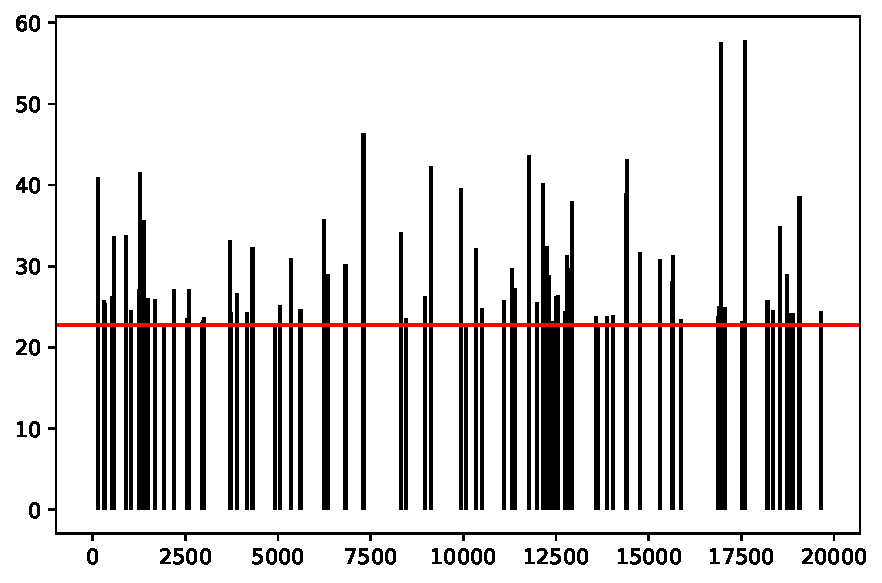
\includegraphics[width=0.7\linewidth]{../plots/ppp-data.pdf}
	\caption{Data in Poisson point process simulation study with
		threshold $u = 22.778$ in red}
	\label{fig:ppp-data}
\end{figure}
%

%
We constructed the priors
with the knowledge of the true quantiles and quantile differences.
Fixing $p = (0.1, 0.01, 0.001)$, then
%
\begin{align*}
	q^*_1 = 39.211 \,, \quad q^*_2 = 62.734 \,, \quad q^*_3 = 99.517 \\
	\implies \tilde{q}^*_1 = 39.211 \,, \quad \tilde{q}^*_2 = 23.523 \,,
		\quad \tilde{q}^*_3 = 36.783
\end{align*}
%
are the true quantiles and quantile differences respectively.
To construct $\pi^{\text{QD}}_q$, we chose
%
\begin{align*}
	\tilde{q}_i \sim \Gamma\left(\frac{(\tilde{q}^*_i) ^ 2}{v},
		\frac{\tilde{q}^*_i}{v}\right) \,, \quad i = 1, 2, 3\\
	\implies \E(\tilde{q}_i) = \tilde{q}^*_i, \quad \Var(\tilde{q}_i) = v
\end{align*}
%
for $v=100$.
%

%
The univariate and bivariate marginals of the priors are illustrated
in Table~\ref{table:ppp-1-marg}, Table~\ref{table:ppp-2-marg},
and Table~\ref{table:ppp-3-marg}.
For $\pi^{\text{SAS}}$, the posterior mean of $\gamma$ was $0.467$.
We plotted the mean return level compared to the analytic true return level
in Fig.~\ref{table:ppp-post-return-level}.
The dashed line was obtained by simulating $270,\!000$ years of data
and calculating the empirical quantiles.
%
\allmarginals{ppp}{Poisson process simulation study}
\allreturnlevels{ppp}{Poisson process simulation study}
%
\subsection{PD: Pseudo-data}
%

%
In order to compare our results to Coles et al.~\cite{coles1996},
we generated data, denoted $\mathbf{x}^{\text{PD}}$,
from $\operatorname{GEV}(17, 1.8, 0.28)$ to resemble their data, such that:
%
\begin{align*}
	\centering
	\renewcommand{\arraystretch}{1.2}
	\begin{tabular}{@{}ccc@{}}
		\toprule[0.1em]
		&$\mathbf{x}^{\text{PD}}$ &Coles et al.\\
		\midrule[0.1em]
		$M$ &$54$ &$54$ \\
		$u$ &$40.109$ &$40$ \\
		$n_u$ &$86$ &$86$ \\
		\bottomrule[0.1em]
	\end{tabular}
\end{align*}
%
This dataset is illustrated in Fig.~\ref{fig:pd-data}.
%
\begin{figure}
	\centering
	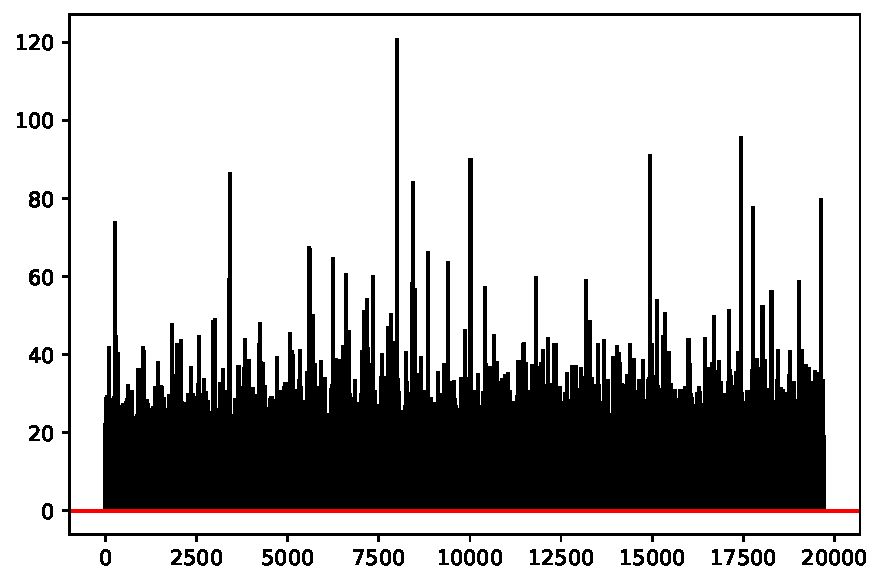
\includegraphics[width=0.7\linewidth]{../plots/pd-data.pdf}
	\caption{Data in pseudo-data simulation study with
		threshold $u = 40.109$ in red}
	\label{fig:pd-data}
\end{figure}
%

%
We used the same prior $\pi^{\text{QD}}_{\tilde{q}}$
for independent quantile differences as specified by Coles et al., given by
%
\begin{align*}
	p &= (0.1, 0.01, 0.001) \,,\\
	\tilde{q}_1 &\sim \Gamma(38.9, 0.67) \,,\\
	\tilde{q}_2 &\sim \Gamma(7.1, 0.16) \,,\\
	\tilde{q}_3 &\sim \Gamma(47, 0.39) \,.
\end{align*}
%

%
The univariate and bivariate marginals of the priors are
illustrated in Table~\ref{table:pd-1-marg}, Table~\ref{table:pd-2-marg},
and Table~\ref{table:pd-3-marg}.
For $\pi^{\text{SAS}}$, the posterior mean of $\gamma$ was $0.638$.
In Table~\ref{table:pd-validation},
we compare the statistics of the quantile differences
specified by the expert, to the statistics estimated
using the MCMC samples of $(\mu, \sigma, \xi)$ for each of the priors.
In Fig.~\ref{table:pd-post-return-level},
the mean return level is plotted with 95\% credibility intervals
and empirical quantiles. 
The dashed black line was obtained by simulating $270,\!000$ years of data
and calculating the empirical quantiles.
We know that the annual maximum has CDF $F^{365}$,
where $F$ is the CDF of $\operatorname{GEV}(17, 1.8, 0.28)$,
and the solid black line shows
the quantiles calculated analytically from this CDF.
%
%\marginals{pd}{theta}{pseudo-data simulation study}
%\marginals{pd}{q}{pseudo-data simulation study}
%
\begin{table*}
	\centering
	\renewcommand{\arraystretch}{1.2}
	\begin{tabular}{@{}ccccc@{}}
		\toprule[0.1em]
		&$\tilde{q}_1$ &$\tilde{q}_2$ &$\tilde{q}_3$ \\
		\midrule[0.1em]
		Expert &(57.563, 70.263) &(42.310, 66.805) &(119.09, 142.836) \\
		$\pi_{\theta}^{\text{QD}}$
			&(57.592, 70.239) &(41.652, 65.907) &(119.868, 143.807) \\
		$\pi_{\theta}^{\text{ME}}$
			&(57.774, 70.694) &(42.601, 71.7) &(121.04, 162.726) \\
		$\pi_{\theta}^{\text{ULS}}$
			&(57.611, 70.266) &(42.191, 66.498) &--- \\
		$\pi_{\theta}^{\text{SAS}}$ &(54.696, 67.987)
			&(26.169, 58.588) &(79.505, 135.024) \\
		\bottomrule[0.1em]
	\end{tabular}
	\caption{Pairs of (median, $0.9$-quantile) of quantile differences 
		for pseudo-data simulation study}
	\label{table:pd-validation}
\end{table*}
%
% \allreturnlevels{pd}{pseudo-data process simulation study}
%

%
In Fig.~\ref{fig:pd-vt}, we varied the threshold,
and plotted the number of exceedances against the return level
for return periods $10^2$, $10^3$, and $10^4$,
all estimated using the prior
$\pi_{\theta \mid \mathbf{x}^{\text{PD}}}^{\text{QD}}$.
%
\begin{figure}
	\centering
	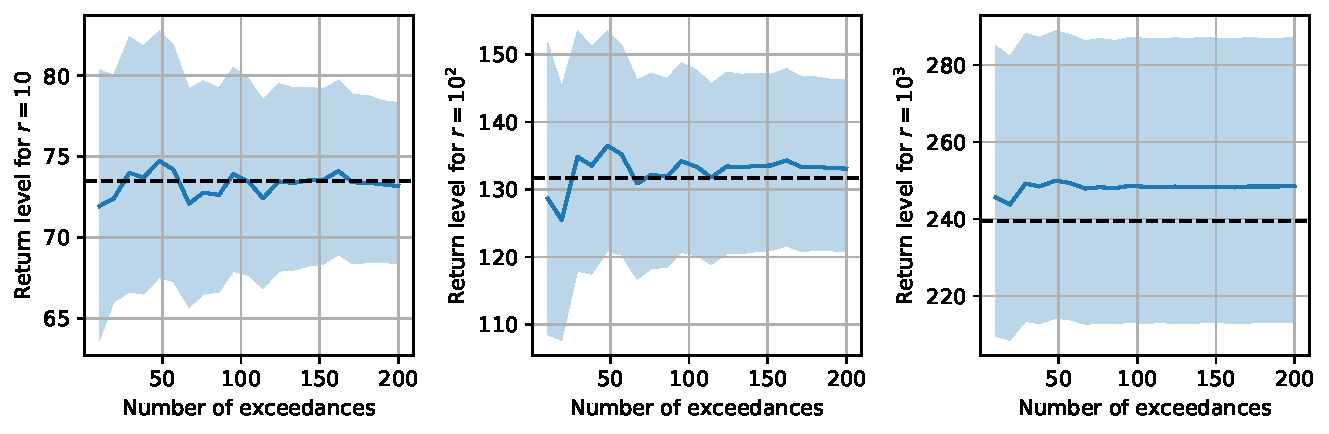
\includegraphics[width=0.9\linewidth]{../plots/pd-vt.pdf}
	\caption{Mean return levels {\color{blue} \textbf{(blue)}}
		with 95\% credibility intervals
		estimated using $\pi_{\theta \mid \mathbf{x}^{\text{PD}}}^{\text{QD}}$
		for various thresholds,
		with simulated return levels {\color{black} \textbf{(black dashed)}}}
	\label{fig:pd-vt}
\end{figure}
%
\subsection{WS: Daily average wind speed at Tours}
%

%
The data in Fig.~\ref{fig:ws-data} represents daily average wind speed at Tours
over a period of X years, from 1981 to 2011. We chose a threshold of $u = 0$.
%
\begin{figure}
	\centering
	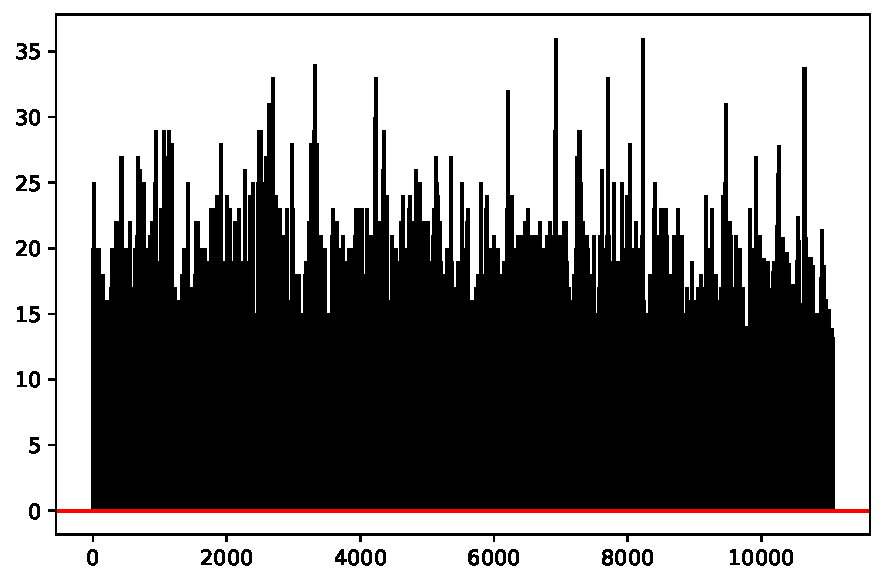
\includegraphics[width=0.7\linewidth]{../plots/ws-data.pdf}
	\caption{Daily average wind speed at Tours with
		threshold $u = 0$ in red}
	\label{fig:ws-data}
\end{figure}
%
\section{Conclusion}
%

%
...
%
\section{Appendix}
%

%
\subsection{Condition (C2) of the maximum entropy distribution
	for Weibull and Gamma distributed marginals}
\label{section:C2}
%
The construction of the maximum entropy distribution in
\S~\ref{section:prior-me} requires the following condition on the marginals:
for a sequence of distributions $(F_i)_{1 \geq i \geq d}$,
%
\begin{align*}
	\textit{(C2)} \coloneqq \forall 1 \leq i \leq d - 1
		\ \forall x \in \{x \colon 1 > F_i(x), F_{i + 1}(x) > 0\}
		\ (F_i(x) > F_{i + 1}(x))\,.
\end{align*}
%
We will investigate this condition for Weibull and Gamma distributed marginals.
%
\subsubsection{Weibull distribution}
%
Let $1 \leq i \leq d - 1$. We have that
%
\begin{align*}
	1 > F_i(x), F_{i + 1}(x) > 0 \iff x > 0 \,.
\end{align*}
%
The CDF when $x > 0$ is
%
\begin{align*}
	F_i(x) = 1 - \exp\left(-\left(\frac{x}{\lambda_i}\right) ^ {k_i}\right) \,,
\end{align*}
%
with $k_i$, $\lambda_i > 0$. Let $ x> 0$. Then
%
\begin{align*}
	\textit{(C2)} & \iff 1 - \exp\left(-\left(\frac{x}{\lambda_i}\right)
		^ {k_i}\right) > 1- \exp\left(-\left(\frac{x}{\lambda_{i + 1}}\right)
		^ {k_{i + 1}}\right)\\
	&\iff \left(\frac{x}{\lambda_i}\right) ^ {k_i} >
		\left(\frac{x}{\lambda_{i + 1}}\right) ^ {k_{i + 1}} \,.
\end{align*}
%
If $k_i = k_{i + 1} = k$,
%
\begin{align*}
	\left(\frac{x}{\lambda_i}\right) ^ k
		> \left(\frac{x}{\lambda_{i + 1}}\right) ^ k&
		\iff \frac{x}{\lambda_i} > \frac{x}{\lambda_{i + 1}}\\
	&\iff \frac{1}{\lambda_i} > \frac{1}{\lambda_{i + 1}}\\
	&\iff \lambda_i < \lambda_{i + 1} \,.
\end{align*}
%
If $k_i \neq k_{i + 1}$,
%
\begin{align*}
	F_i(x) =F_{i + 1}(x)
		&\iff \left(\frac{x}{\lambda_i}\right) ^ {k_i}
		= \left(\frac{x}{\lambda_{i + 1}}\right) ^ {k_{i + 1}}\\
	&\iff \exp\left(k_i (\log x - \log\lambda_i)\right)
		=\exp\left({k_{i + 1}}(\log x - \log\lambda_{i + 1})\right)\\
	&\iff k_i (\log x - \log\lambda_i)
		= {k_{i + 1}} (\log x - \log\lambda_{i + 1})\\
	&\iff k_i \log x - k_i \log\lambda_i 
		= {k_{i + 1}} \log x - {k_{i + 1}} \log\lambda_{i + 1}\\
	&\iff k_i \log x - {k_{i + 1}} \log x
		=k_i \log\lambda_i - {k_{i + 1}} \log\lambda_{i + 1}\\
	&\iff (k_i - {k_{i + 1}}) \log x 
		= k_i \log\lambda_i - {k_{i + 1}} \log\lambda_{i + 1}\\
	&\iff \log x
		= \frac{k_i \log\lambda_i - {k_{i + 1}}
		\log\lambda_{i + 1}}{k_i - {k_{i + 1}}}\\
	&\iff x
		= \exp\underbrace{\left(\frac{k_i \log\lambda_i - {k_{i + 1}}
		\log\lambda_{i + 1}}{k_i - {k_{i + 1}}}\right)}
		_{\eqqcolon h(k_i, \lambda_i, k_{i + 1}, \lambda_{i + 1})} \,.
\end{align*}
%
Therefore the two CDFs intersect, and so $\textit{(C2)}$ cannot be satisfied.
In conclusion,
%
\begin{align*}
	\textit{(C2)}
		&\iff (k_i = k_{i + 1}) \land (\lambda_i < \lambda_{i + 1})
		\quad \forall 1 \leq i \leq d - 1 \,.
\end{align*}
%

%
In practice however, as
$y \coloneqq h(k_i, \lambda_i, k_{i+1}, \lambda_{i+1}) \to \pm \infty$,
the intersection will tend to the bounds of the set
$\{x \colon 1 > F_i(x), F_{i + 1}(x) > 0\}$ and so $\textit{(C2)}$
will be asymptotically satisfied. When does this happen?
Consider a reparametrisation
%
\begin{align*}
	(k_i, \lambda_i, k_{i + 1}, \lambda_{i + 1}) \mapsto
		(k_i, \lambda_i, k_i - {k_{i + 1}}, \lambda_{i + 1}) \,,
\end{align*}
%
which implies that
%
\begin{align*}
	h(k_i, \lambda_i, z_{i}, \lambda_{i+1})
		=\frac{k_i \log\lambda_i + {(z_{i} - k_{i})}
		\log\lambda_{i + 1}}{z_{i}} \,,
		\quad z_{i} < k_i,\ z_{i} \neq 0 \,.
\end{align*}
%
Then
%
\begin{itemize}
	\item As $z_i \to 0$, $y \to +\infty$,
	\item As $k_i \to +\infty$, $y \to \pm\infty$, with sign depending
		on the sign of $\log(\frac{\lambda_i}{\lambda_{i + 1}})$,
	\item As $\lambda_i \to +\infty$ or $\lambda_{i + 1} \to 0$,
		$y \to +\infty$,
	\item As $\lambda_i \to 0$ or  $\lambda_{i + 1}\to +\infty$,
		$y \to -\infty$.
\end{itemize}
%
\subsubsection{Gamma distribution}
%

%
Let $1 \leq i \leq d - 1$. We have that
%
\begin{align*}
	1 > F_i(x), F_{i+1}(x) > 0 \iff x > 0 \,.
\end{align*}
%
Suppose that we have two such distributions,
%
\begin{align*}
	F_1(x) = \frac{\beta^{\alpha_1}_1}{\Gamma(\alpha_1)} x ^ {\alpha_1}
	\exp(\beta_1 x) \quad \text{and} \quad
	F_2(x) = \frac{\beta^{\alpha_2}_2}{\Gamma(\alpha_2)} x ^ {\alpha_2}
	\exp(\beta_2 x) \,,
\end{align*}
%
with $\alpha_i, \beta_i>0$ the shape and rate parameters.
Denote their respective PDFs by $f_1$ and $f_2$.
Let $x > 0$, and define
%
\begin{align*}
	\phi(x) = F_2(x) - F_1(x) \,,
\end{align*}
%
so that if $(i, i + 1) = (1, 2)$,
%
\begin{align*}
	\textit{(C2)} \iff \phi(x) < 0 \,,
\end{align*}
%
and if $(i, i + 1) = (2, 1)$,
%
\begin{align*}
	\textit{(C2)} \iff \phi(x) > 0 \,.
\end{align*}
%
We have that
%
\begin{align*}
	\phi'(x) &= f_2(x) - f_1(x)\\
	&= f_1(x) \left(\frac{f_2(x)}{f_1(x)} - 1\right)\\
	&= f_1(x) \left(\frac{\Gamma(\alpha_1)\beta ^ {\alpha_2}_2}
		{\Gamma(\alpha_2)\beta ^ {\alpha_1}_1} x^{\alpha_2 - \alpha_1}
		\exp((\beta_1 - \beta_2) x) - 1\right) \,.
\end{align*}
%
Let
%
\begin{align*}
	C \coloneqq \frac{\Gamma(\alpha_1) \beta ^ {\alpha_2}_2}
		{\Gamma(\alpha_2) \beta ^ {\alpha_1}_1} > 0
\end{align*}
%
and
%
\begin{align*}
	f(x) \coloneqq C x ^ {\alpha_2 - \alpha_1}
		\exp((\beta_1 - \beta_2) x) - 1 \,.
\end{align*}
%
Then
%
\begin{align*}
	f'(x) &= C\left[(\alpha_2 - \alpha_1) x ^ {\alpha_2 - \alpha_1 - 1}
		\exp((\beta_1 - \beta_2) x) + x ^ {\alpha_2 - \alpha_1}
		\exp((\beta_1 - \beta_2) x)(\beta_1 - \beta_2) \right]\\
	&=\underbrace{C x ^ {\alpha_2 - \alpha_1 - 1} \exp((\beta_1 - \beta_2) x)}
		_{ > 0} \left[(\alpha_2 - \alpha_1) + x (\beta_1 - \beta_2)\right]
\end{align*}
%
\subsubsection*{\underline{Case 1:
	$(\alpha_1\leq\alpha_2\land \beta_1\geq\beta_2)
	\land\neg(\alpha_1=\alpha_2\land\beta_1=\beta_2)$}}
%

%
We have that $\alpha_2 - \alpha_1 \geq 0$ and
$\beta_1 - \beta_2 \geq 0$, and therefore
%
\begin{align*}
	(\alpha_2 - \alpha_1) + x(\beta_1 - \beta_2) &> 0\\
	\implies f'(x) & > 0 \,.
\end{align*}
%
This implies that $f$ is strictly increasing on $\R^+$.
%
\begin{enumerate}
	\item If $\alpha_1 < \alpha_2$, we have that
		\begin{align*}
			\lim_{x \to 0^+} f(x) = -1 \quad \text{and} \quad
				\lim_{x \to +\infty} f(x) = +\infty\,.
		\end{align*}
	\item If $\alpha_1 = \alpha_2 = \alpha$ and $\beta_1 > \beta_2$,
		we have that
		\begin{align*}
			\lim_{x \to 0^+} f(x)
				= \left(\frac{\beta_2}{\beta_1}\right) ^ \alpha - 1 < 0 \quad
				\text{and} \quad \lim_{x \to +\infty} f(x) = +\infty \,.
		\end{align*}
\end{enumerate}
%
Therefore in both cases, there exists a unique $z_0 > 0$
such that $f(z_0) = 0$. This implies that
%
\begin{align*}
	\begin{cases}
		\phi'(x) < 0 &\text{if} \quad x < z_0 \,,\\
		\phi'(x) = 0 &\text{if} \quad x = z_0 \,,\\
		\phi'(x) > 0 &\text{if} \quad x > z_0 \,.
	\end{cases}
\end{align*}
%
In order to proceed we will need the following Lemma.
%
\begin{lemma}
	\begin{enumerate}
		\item Let $f \colon (a, b] \to \R$ be continuous on $(a, b]$
			and differentiable on $(a, b)$, with 
			$a \in \R \cup \{+\infty\}, b \in \R$. If for all $x \in (a, b)$,
			\ $f'(x) > 0$ (resp. $<$) and $\lim_{x \to a^+} f(x) = L \in \R$,
			then for all $z \in (a, b]$, $f(z) > L$ (resp. $<$).
		\item Let $f \colon [a, b) \to \R$ be continuous on $[a, b)$
			and differentiable on $(a, b)$, with
			$a \in \R, b \in \R \cup \{+\infty\}$. If for all $x\in(a, b)$,
			\ $f'(x) > 0$ (resp. $<$) and $\lim_{x \to b^-} f(x) = L \in \R$,
			then for all $z \in [a, b)$, $f(z) < L$ (resp. $>$).
	\end{enumerate}
	\label{limit}
\end{lemma}
%
\begin{proof}
	We will prove the first case, for $f'(x) > 0$,
	as both cases are symmetrical. Suppose that $z \in (a, b)$.
	We need to show that $f(z),f(b) > L$. Let $y \in (a, z)$.
	As $f'$ is strictly positive on $(a, b)$, $f$ is strictly increasing
	(by the mean value theorem), and so $f(z) - f(y) = c > 0$.
	Therefore $f(z) > f(y) + \frac{c}{2}$.
	Then $f(z) = \lim_{y \to a^+} f(z) \geq \lim_{y \to a^+} f(y)
	+ \frac{c}{2} = L + \frac{c}{2} > L$.
	Furthermore, $f(b) = \lim_{z \to b^-} f(z) \geq \lim_{x \to b^-} 
	(L + \frac{c}{2}) = L + \frac{c}{2} > L$.
\end{proof}
%

%
By Lemma \ref{limit}, for all $z \in (0, z_0]$,
$\phi(z) < \lim_{x\to 0^+}\phi(x)=0$, and for all $z \in[z_0, +\infty)$,
$\phi(z) < \lim_{x \to +\infty} \phi(x) = 0$.
Therefore for all $x > 0$, $\phi(x) < 0$, and so if $(i, i + 1)=(1, 2)$,
(C2) is satisfied, and if $(i, i + 1) = (2, 1)$, (C2) is violated.
%
\subsubsection*{\underline{Case 2: $\alpha_1<\alpha_2,\  \beta_1<\beta_2$}}
%

%
Since
%
\begin{align*}
	\lim_{x \to 0^+} f(x) = -1 \,,
\end{align*}
%
there exists a $\delta > 0$ such that for all $z \in (0, \delta]$,
$f(z) = \phi'(z) < 0$, and so by Lemma \ref{limit},
$\phi(z) < \lim_{x \to 0^+} \phi(x) = 0$. Since
%
\begin{align*}
	\lim_{x \to +\infty} f(x) = -1 \,,
\end{align*}
%
there exists a $\delta' > 0$ such that for all $z \in [\delta', +\infty)$,
$f(z) = \phi'(z) < 0$, and so by Lemma \ref{limit},
$\phi(z) > \lim_{x \to 0^+} \phi(x) = 0$.
Therefore $\phi$ is neither strictly positive nor strictly negative,
and so if either $(i, i + 1) = (1, 2)$ or
$(i, i + 1) = (2, 1)$, (C2) is violated.
%

%
In conclusion, we have shown that
%
\begin{align*}
	\textit{(C2)} \iff (\alpha_i \leq \alpha_{i + 1} \land \beta_{i}
	\geq \beta_{i + 1}) \land \neg(\alpha_i = \alpha_{i+1} \land \beta_i
	= \beta_{i + 1}) \quad \forall 1 \leq i\leq d - 1 \,.
\end{align*}
%
Like in the Weibull case, the condition can be asymptotically satisfied.
For instance, if the means $\frac{\alpha}{\beta}$ are sufficiently separated,
and the variances $\frac{\alpha}{\beta ^ 2}$ are small,
there will be less significant overlap between the CDFs.
%
\metroall{pd}{PD}{pseudo-data simulation study}
\metroall{ppp}{PPP}{Poisson process simulation study}
%
\bibliography{mybib}
\bibliographystyle{plain}
%
\end{document}